\FloatBarrier
\section{Soft Cut Detection}
\label{sec:soft_cut}

% To occur somewhere in this chapter:
% \begin{itemize}
%     \item Test with 11 frame length and 21 frame length
%     \item Test with only lstms, only basic CNN before (intuition: CNN is not so good anyways)
%     \item One-LSTM vs. Two-LSTMs
%     \item All the different merges. Why merge at all?
%     \item Evaluate on sequence and on frame level?
%     \item Histograms for debugging?
%     \item Why it did not work out.

% \end{itemize}
%%%
%%% Hier mal noch die Ideen, die wir irgendwann hatten fuer soft-cut und hard-cut. Vllt kann man Teile davon noch irgendwo einbauen.
%%%

%- Hard Cut Detection: Visualisierungen
%  Verbesserungsideen:  - Hinzunahme der vorherigen Frames
%                       - Edges
%                       - Subraktion der beiden Frames -> einfarbiges Bild?
%                       - Trainingsverhältnis
%                       - 2007
%- Soft Cut Generierung
%- Soft Cut Detection:
%  Frage:   - Wie soll der Input aussehen? Einzelne Frames. Erkennen von Fade In/Out durch das Schwarzerwerden.
%           - Erkennen von Dissolves durch das Überlappen zweier Frames.
%           - Reine Pixel als input
%           - Preprocessing? Komprimierung der Frames?
%
%           - Input Size: 10 Frames
%           - Training: Fix Länge, klein
%                       Auf selbst generierten Daten
%           - Test: True -> rechts und links schauen
%                           Sozusagen schrittweise ueber das Video gehen, und jeweils 5 Frames links und rechts mit in das Sliding Window nehmen.
%                           Wenn mehrfach nacheinander ein dissolve vorausgesagt wird
%
%                   Test auf 2007er Daten


In contrast to the traditional approaches presented in Section~\ref{sec:related_work}, we chose a deep learning approach to detect soft cuts in a video.
In the following subsections, this approach is presented in more detail.

\subsection{Data Generation}
\label{sec:soft_cut_data_generation}

After having trained a recurrent neural net with the existing data, we noticed that the net did not generalize very well.
In order to solve this problem, more data was necessary.
We decided to generate more data by blending random sequences into each other.
A random sequence is picked by reading the gold standard, picking two consecutive elements which encode two cuts with a start and end frame each.
Between the end frame of the first cut and the start frame of the first cut, we can randomly select a subsequence with the desired transition length (11 and 21).
In order to blend two random sequences, we have multiple options for tweening behaviour.
The standard tweening function is linear, but there are also EaseIn, EaseOut etc. (see Figure~\ref{fig:data_generation}).
The tweening function is randomly selected, as well.

In order to achieve further variance in the generated data, we flip the two sequences randomly at the x- or y-axis or at both axes.
With this approach we generated 50 GB of data.


\begin{figure}
    \centering
    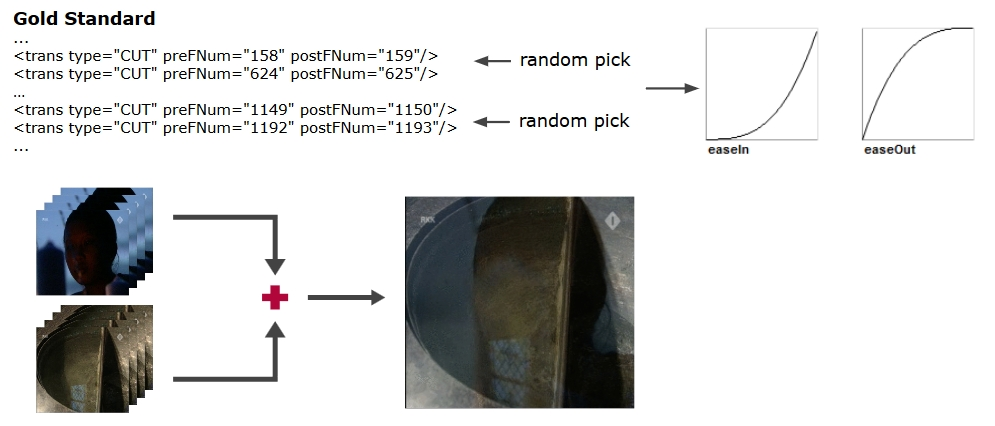
\includegraphics[scale=.5]{images/data_generation.jpg}
    \caption{}
    \label{fig:data_generation}
\end{figure}
\subsection{Approach}
\label{sec:soft_cut_approach}

For the soft cut detection we decided to use a deep learning approach.
More concretely, we used the RNN/LSTM implementation by Jeff Donahue\footnote{\url{https://github.com/BVLC/caffe/pull/2033}} for the Caffe\footnote{\url{http://caffe.berkeleyvision.org/}} framework.
This RNN/LSTM implementation takes two different inputs: On the one hand the raw pixel values and on the other hand a tagging sequence.
The tagging sequence tells the LSTM, where a new training example starts, as we process more than one training sequence per batch.
The LSTM implementation allows us to use a short term memory in the neural network.
The network remembers information from the beginning of a frame sequence until the last frame of the sequence.
So the net remembers previous decisions through a sequence of frames.

But using this architecture has one problem, as stated by Jeff Donahue: ``Backpropagation [through the LSTM] is truncated along the batch boundaries''. % \textcolor{red}{TODO}: Quelle.
So one or more frame sequences have to fit exactly into the batch size used by the RNN/LSTM.
This is hard to achieve, if we want to classify variable-length frame sequences.
Therefore we decided to use a fixed size for the sequences of frames in our training data, i.e. we would generate only transitions of length ten in our training data.

However, we still want to find soft cuts of arbitrary length in a video.
To achieve this, we repeatedly test fixed-size frame sequences.
In Figure~\ref{fig:soft_cut_approach}, we show an example.
\begin{figure}[!htb]
	\centering
	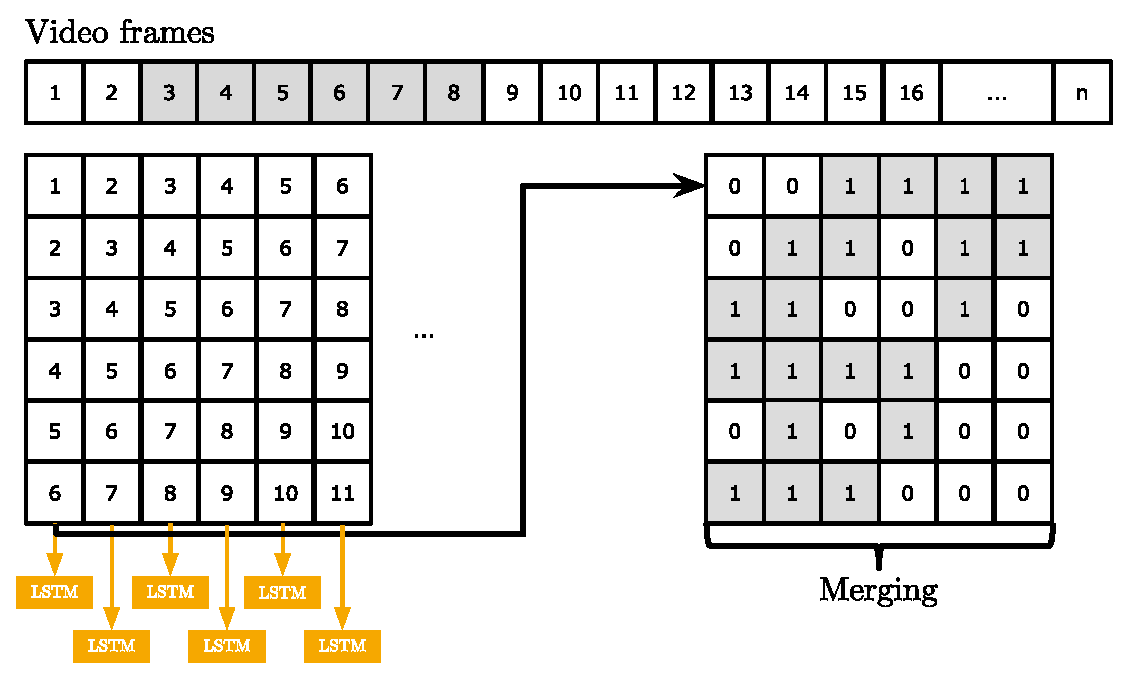
\includegraphics[scale=.7]{images/soft_cut_approach.eps}
	\caption{To classify soft cuts of arbitrary length, we repeatedly test fixed-size frame sequences. In this example we test sequences of size six. Afterwards the predictions given by the RNN/LSTM are merged, so that we have one prediction per frame.}
	\label{fig:soft_cut_approach}
\end{figure}
We have a video with \textit{n} frames.
The frames from three to eight represent a soft cut.
Now, for each frame, we generate a frame sequence of size six starting from that frame.
This is equivalent to moving a sliding window over the frames.
Those sequences are then classified by the RNN/LSTM.
The output of the RNN/LSTM is zero, if a frame does not belong to a soft cut, and one, otherwise.
In the end, we have six predictions per frame, which have to be merged, so that we have only one prediction per frame.
After merging, consecutive frames with a predicted value of 1 represent one soft cut.

In the following several strategies for combining multiple frame predictions into one prediction are presented.
An overview over all strategies can be found in Figure~\ref{fig:merging_strategies}.
\begin{figure}[!htb]
	\centering
	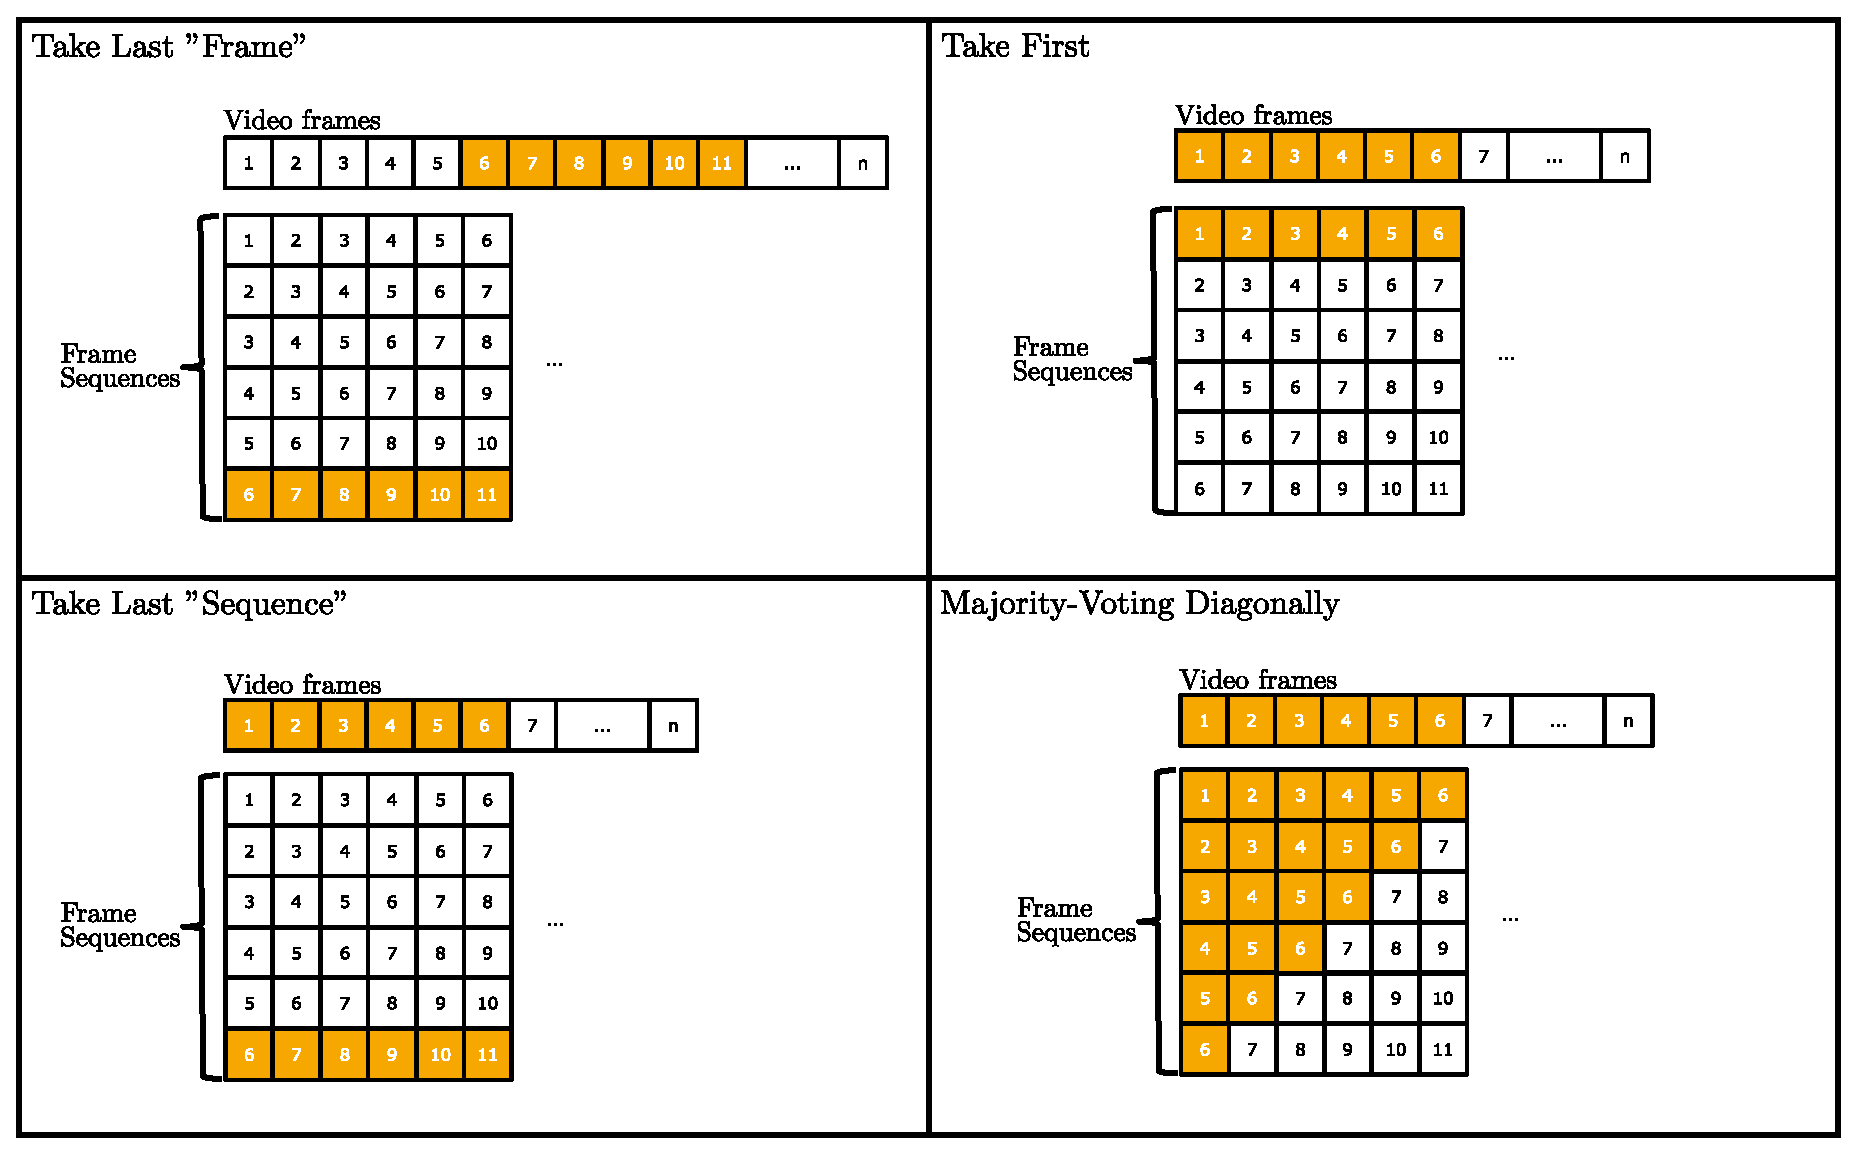
\includegraphics[scale=.5]{images/merging_strategies.eps}
	\caption{To merge the multiple predictions per frame into one, we implemented several strategies:
    \textit{Take Last 'Frame'} (top left): The prediction of the frame, where the frame is the last of a frame sequence, is taken.
    \textit{Take Last 'Sequence'} (bottom left): The last prediction of the frame sequence belonging to a frame is taken.
    \textit{Take First} (top right): The first prediction of the frame sequence is taken.
    \textit{Majority-Voting Diagonally} (bottom right): The majority voting among all predictions of the frame is taken.}
	\label{fig:merging_strategies}
\end{figure}
\paragraph{Take First}
A first simple strategy is to take the first prediction of each sequence as the prediction of that frame.
This is equivalent to having no prior knowledge about the frame, as the RNN/LSTM has not seen any previous frames and therefore could not remember anything.

\paragraph{Take Last 'Sequence'}
A second simple strategy is to take the last prediction of each sequence as the prediction for the frame that started the sequence.
Concretely, the last prediction is not a prediction for the frame under question, but the intuition behind this is that an RNN/LSTM becomes more and more certain after having seen multiple frames of the sequence.

\paragraph{Take Last 'Frame'}
In the \textit{Take Last 'Frame'} strategy, for every frame we take the frame sequence, in which that frame is the last one.
The intuition is similar to the previous case, but now we also use the prediction for the actual frame.

\paragraph{Majority-Voting Diagonally}
Each frame is predicted up to \textit{n} times.
In our example it is up to six times.
In the \textit{Majority-Voting Diagonally} all of those predictions are taken and the majority voting among those is taken as prediction for the frame.
Ties are resolved by placing more weight on the half of the predictions, where the frame appeared later in the sequence.

After merging we have one prediction per frame indicating whether the frame is part of a soft cut or not.
Then, a sequence of frames that are part of a soft cut represents a soft cut.
However, there could be misclassified frame predictions.
We implemented a \textit{Gap Filler} to find and correct some of those misclassified frame predictions.
The \textit{Gap Filler} is looking for sequences of frames that belong to a soft cut and are interrupted by some non cut frames.
If the number of interrupting frames is not too large, they are also classified as soft cut frames.
The idea behind the \textit{Gap Filler} is that two soft cuts do not occur close to each other.
So, if two soft cuts are only a few frames apart, they probably belong to the same soft cut.
In Figure~\ref{fig:gap_filler} an example of the \textit{Gap Filler} is shown.
There, a sequence of soft cut frames is interrupted by two non soft cut frames.
Those non soft cut frames are detected by the \textit{Gap Filler} and classified as soft cut frames.
\begin{figure}[!htb]
	\centering
	
\includegraphics[scale=.7]{images/gap_filler.eps}
	\caption{Two soft cuts do not occur close to each other. Therefore the \textit{Gap Filler} finds misclassified frame predictions after the merging step and corrects non soft cut frame predictions, if they are interrupting a soft cut.}
	\label{fig:gap_filler}
\end{figure}

Another idea for correcting misclassified frame predictions is to delete soft cuts that are only up to five frames long and only surrounded by non soft cut frames.
In our data set a soft cut has an average length of 22 frames.
The smallest have a length of seven frames.
Therefore, a soft cut of only up to five frames is not realistic and misclassified with a high probability.

% \textcolor{red}{TODO}: Ich finde, das sollte doch ein eigener Abschnitt werden, oder?
% Das ist ja jetzt ein komplett anderes Thema auf einmal.
% Und sollte der folgende Teil dann nicht auch zuerst kommen?
% \textcolor{red}{TODO}: Hier muss auch noch hin, we tested many different architectures, and parameters, in the following we present a small selection of that with significant differences.
To classify the frames as soft cut or non soft cut frames, we used an RNN/LSTM.
We tested the following architectures:

\paragraph{CNN + one LSTM}
For the CNN we used the architecture of the \textit{caffenet} [\textcolor{red}{TODO}: reference].
We also used the pre trained weights of this net, so that we do not need to train our model from scratch.
We only fine-tuned the \textit{fc6} layer of the \textit{caffenet} with a learning rate of 0.1.
The CNN is followed by one LSTM, whose weights were initialized with the \textit{Xavier} method [\textcolor{red}{TODO} Zitat: \url{http://jmlr.org/proceedings/papers/v9/glorot10a/glorot10a.pdf}].
Besides, the general learning rate was set to 0.01 and gradient clipping was used.

\paragraph{CNN + two LSTMs}
The architecture of this net is basically the same as the previous.
There is only one difference: Instead of using just one LSTM, two LSTMs were used.
Also the general learning rate was set to 0.001 and no gradient clipping was used.
The architecture of the net can be found in Figure~\ref{fig:net_architecture}.
\begin{figure}[!htb]
	\centering
	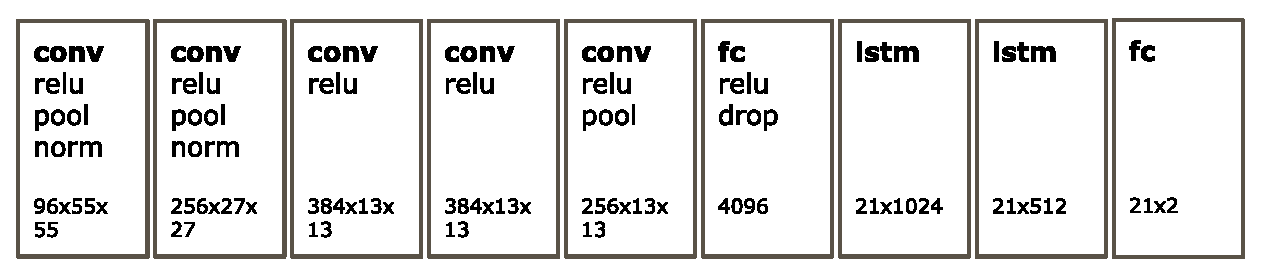
\includegraphics[scale=.5]{images/net_architecture.eps}
	\caption{Architecture of the RNN/LSTM consisting of a CNN and two LSTMs.}
	\label{fig:net_architecture}
\end{figure}

\paragraph{One convolutional layer + two LSTMs}
The last architecture that was tested uses only one convolutional layer before the two LSTMs.
The intuition behind it is as follows: for the CNN, it is hard to detect a soft cut frame, because it works only on one frame.
By looking at only one frame, it would be difficult to predict a soft cut, even for a human.
However, by looking at a sequence of frames, this becomes easier.
This is exactly, what the RNN/LSTM does, which is why we put more emphasis on this part and less emphasis on the CNN part.
The net was trained from scratch as no pretrained net existed.
The weights of the LSTMs were again initialized using the \textit{Xavier} method.
The learning rate was 0.001 and gradient clipping was used during training.


\subsection{Evaluation}
\label{sec:hard_cut_evaluation}

\begin{table}[ht]
	\centering
	\begin{tabular}{l|l}
	Precision & XX \% \\ \hline
	Recall & XX \% \\ \hline
	Accuracy & XX \% \\
	\end{tabular}
	\caption{Results of the hard cut detection}
	\label{tab:hard_cut_results}
\end{table}

\subsubsection{Training Data}
The SVM is trained on an mixture of videos from the 2007 TrecVid contest.
The videos in their full length do not make a good training set, as the ratio between hard cuts and other frames is about \texttt{1:1000}, leading to a failure to predict any hard-cuts.
A custom training set must be constructed, which contains a suffcient amount of hard cuts.
The choice of non-hard-cuts is also crucial for achieving good classification performance: too homogenous frames will lower the decision boundary, and lead to bad performance on noisy examples.
Therefore the negative set should also include soft-cuts and particularly noisy frames.
The training set we finally build consists of about 250 hard cuts and 2200 negatives.

